\chapter{Pruebas y resultados}
	A continuación se detallan las pruebas realizadas y los resultados obtenidos
	por cada módulo desarrollado, utilizando como base los modelos
	\texttt{armadillo}, \texttt{bunny}, \texttt{dragon}, \texttt{drill} y \texttt{happy}
	del repositorio de Stanford\cite{StanfordScanRep}.

	De cada modelo se seleccionaron aquellas capturas que fueron realizadas
	completando una vuelta alredor del objeto.
	Se observa que la distancia entre capturas presenta un mínimo de $24^{\circ}$

	\section{Módulo de registración}
	Para la registración se utilizó el método basado en la búsqueda de clúster,
	seguido de un refinamiento mediante ICP y una corrección de bucle.
	Se plantearon dos métodos para evaluar la calidad de cada registración:
	\begin{itemize}
		\item Mediante la comparación entre la transformación calculada y aquella provista por la base de datos (\emph{ground truth}).
		\item Mediante una métrica de \emph{fitness} que se obtiene a partir de la nube transformada y las nubes de entrada.
	\end{itemize}

	Para comparar las alineaciones contra el \emph{ground truth}, se
	observa el efecto de las mismas sobre un punto orientado simulando la
	cámara (figura~\ref{fig:err_reg}). El punto \emph{eye} ($C$) se ubica inicialmente en las coordenadas
	$\{0, -0.1, 0.7\}$ (valores obtenidos de la base de datos), y se
	orienta el vector \emph{target} hacia $-z$ y el \emph{up} hacia $y$.
	El error de posicionamiento es la razón entre la distancia al punto
	de inicio y la distancia al punto obtenido por el \emph{ground truth}.
	\[\text{Error} = \frac{|C'-C_{gt}|}{|C_{gt} - C|}\]
	Los errores de \emph{target} y \emph{up} se corresponden al ángulo formado contra los
	vectores respectivos obtenidos por el \emph{ground truth}.

	\begin{figure}
		\centering
		\input{diagram/error_registration.pdf_tex}
		\caption{\label{fig:err_reg}Comparación entre las transformaciones de alineación.
		Se observa el efecto producido en un punto orientado $C$ que simula la posición de la cámara.}
	\end{figure}

	En el cuadro~\ref{tab:reg_error} se presentan los errores de registración promedio para cada orientación de los modelos.
	En la mayoría de los casos, los errores no superan $1^{\circ}$ en orientación ni $1\%$ en posicionamiento,
	observándose dos excepciones: \texttt{bunny} y \texttt{dragon stand}.
	El aumento en el error del modelo \texttt{bunny} se debe a que la captura \texttt{bun180} presenta una distancia cercana a $90^\circ$,
	superando las restricciones impuestas en este trabajo.
	Sin embargo, en el caso de \texttt{dragon stand} el error refleja una mala
	alineación en la captura~12, debida a una mala selección de los parámetros.
	Mediante un posterior ajuste de los parámetros, en particular, del tamaño de la vecindad para el cálculo de los descriptores, se obtuvo una alineación correcta.

	\begin{table}
	\centering
	\begin{tabular}{l*{3}{c}}
		\toprule                                                                  
		Modelo                   &    Eye          &    Target (grados)        &    Up (grados)\\
		\midrule
		armadillo back          &     0.0062159   &   0.221725     &    ---\\        
		armadillo head          &     0.0036356  &    0.102321     &    0.211231\\   
		armadillo head offset   &     0.0029806  &    0.086309     &    0.229574\\   
		armadillo stand         &     0.0022145  &    0.049612     &    0.105862\\   
		armadillo stand flip    &     0.0045019  &    0.125330     &    0.146033\\   
		\midrule
		bunny                   &     0.0104809   &   0.598354     &    0.817185\\   
		\midrule
		dragon side             &     0.0070872  &    0.178650     &    0.212932\\   
		dragon stand            &     0.0536199   &   1.379760     &    0.207754\\   
		dragon up               &     0.0058265  &    0.139297     &    ---\\        
		\midrule
		drill                   &     0.0082317  &    0.238639     &    0.100126\\   
		\midrule
		happy back              &     0.0088540  &    0.189885     &    0.207247\\   
		happy side              &     0.0072675   &   0.175860     &    ---\\        
		happy stand             &     0.0050124  &    0.101383     &    0.097800\\  
		\bottomrule                                                               
	\end{tabular}
	\caption[Errores de registración]{\label{tab:reg_error}Errores de registración.
	\TODO{¿por qué hay vacíos?}}
\end{table}


	Para evaluar la alineación entre un par de capturas prescindiendo del \emph{ground truth}, y situándonos en un escenario más realista,
	se diseñó una medida de \emph{fitness}.
	Esta medida se define como el porcentaje del área solapada entre las nubes una vez alineadas,
	donde un bajo solapamiento nos indicaría un posible error de alineación, como
	se observa en la figura~\ref{fig:fitness}.

	\begin{figure}
		\centering
			\begin{tikzpicture}[gnuplot]
%% generated with GNUPLOT 5.4p0 (Lua 5.4; terminal rev. Jun 2020, script rev. 114)
%% Tue 25 Aug 2020 01:55:34 AM -03
\gpmonochromelines
\path (0.000,0.000) rectangle (12.500,8.750);
\gpcolor{color=gp lt color border}
\gpsetlinetype{gp lt border}
\gpsetdashtype{gp dt solid}
\gpsetlinewidth{1.00}
\draw[gp path] (1.320,0.985)--(1.500,0.985);
\draw[gp path] (11.947,0.985)--(11.767,0.985);
\node[gp node right] at (1.136,0.985) {$0$};
\draw[gp path] (1.320,2.476)--(1.500,2.476);
\draw[gp path] (11.947,2.476)--(11.767,2.476);
\node[gp node right] at (1.136,2.476) {$0.2$};
\draw[gp path] (1.320,3.967)--(1.500,3.967);
\draw[gp path] (11.947,3.967)--(11.767,3.967);
\node[gp node right] at (1.136,3.967) {$0.4$};
\draw[gp path] (1.320,5.459)--(1.500,5.459);
\draw[gp path] (11.947,5.459)--(11.767,5.459);
\node[gp node right] at (1.136,5.459) {$0.6$};
\draw[gp path] (1.320,6.950)--(1.500,6.950);
\draw[gp path] (11.947,6.950)--(11.767,6.950);
\node[gp node right] at (1.136,6.950) {$0.8$};
\draw[gp path] (1.320,8.441)--(1.500,8.441);
\draw[gp path] (11.947,8.441)--(11.767,8.441);
\node[gp node right] at (1.136,8.441) {$1$};
\draw[gp path] (1.984,0.985)--(1.984,1.165);
\draw[gp path] (1.984,8.441)--(1.984,8.261);
\node[gp node center] at (1.984,0.677) {1};
\draw[gp path] (2.648,0.985)--(2.648,1.165);
\draw[gp path] (2.648,8.441)--(2.648,8.261);
\node[gp node center] at (2.648,0.677) {2};
\draw[gp path] (3.313,0.985)--(3.313,1.165);
\draw[gp path] (3.313,8.441)--(3.313,8.261);
\node[gp node center] at (3.313,0.677) {3};
\draw[gp path] (3.977,0.985)--(3.977,1.165);
\draw[gp path] (3.977,8.441)--(3.977,8.261);
\node[gp node center] at (3.977,0.677) {4};
\draw[gp path] (4.641,0.985)--(4.641,1.165);
\draw[gp path] (4.641,8.441)--(4.641,8.261);
\node[gp node center] at (4.641,0.677) {5};
\draw[gp path] (5.305,0.985)--(5.305,1.165);
\draw[gp path] (5.305,8.441)--(5.305,8.261);
\node[gp node center] at (5.305,0.677) {6};
\draw[gp path] (5.969,0.985)--(5.969,1.165);
\draw[gp path] (5.969,8.441)--(5.969,8.261);
\node[gp node center] at (5.969,0.677) {7};
\draw[gp path] (6.634,0.985)--(6.634,1.165);
\draw[gp path] (6.634,8.441)--(6.634,8.261);
\node[gp node center] at (6.634,0.677) {8};
\draw[gp path] (7.298,0.985)--(7.298,1.165);
\draw[gp path] (7.298,8.441)--(7.298,8.261);
\node[gp node center] at (7.298,0.677) {9};
\draw[gp path] (7.962,0.985)--(7.962,1.165);
\draw[gp path] (7.962,8.441)--(7.962,8.261);
\node[gp node center] at (7.962,0.677) {10};
\draw[gp path] (8.626,0.985)--(8.626,1.165);
\draw[gp path] (8.626,8.441)--(8.626,8.261);
\node[gp node center] at (8.626,0.677) {11};
\draw[gp path] (9.290,0.985)--(9.290,1.165);
\draw[gp path] (9.290,8.441)--(9.290,8.261);
\node[gp node center] at (9.290,0.677) {12};
\draw[gp path] (9.954,0.985)--(9.954,1.165);
\draw[gp path] (9.954,8.441)--(9.954,8.261);
\node[gp node center] at (9.954,0.677) {13};
\draw[gp path] (10.619,0.985)--(10.619,1.165);
\draw[gp path] (10.619,8.441)--(10.619,8.261);
\node[gp node center] at (10.619,0.677) {14};
\draw[gp path] (11.283,0.985)--(11.283,1.165);
\draw[gp path] (11.283,8.441)--(11.283,8.261);
\node[gp node center] at (11.283,0.677) {0};
\draw[gp path] (1.320,8.441)--(1.320,0.985)--(11.947,0.985)--(11.947,8.441)--cycle;
\node[gp node center,rotate=-270] at (0.292,4.713) {solapamiento};
\node[gp node center] at (6.633,0.215) {captura};
\draw[gp path] (1.873,0.985)--(1.873,8.158)--(2.095,8.158)--(2.095,0.985)--cycle;
\draw[gp path] (2.538,0.985)--(2.538,8.144)--(2.759,8.144)--(2.759,0.985)--cycle;
\draw[gp path] (3.202,0.985)--(3.202,6.102)--(3.423,6.102)--(3.423,0.985)--cycle;
\draw[gp path] (3.866,0.985)--(3.866,6.882)--(4.087,6.882)--(4.087,0.985)--cycle;
\draw[gp path] (4.530,0.985)--(4.530,5.745)--(4.752,5.745)--(4.752,0.985)--cycle;
\draw[gp path] (5.194,0.985)--(5.194,7.078)--(5.416,7.078)--(5.416,0.985)--cycle;
\draw[gp path] (5.859,0.985)--(5.859,7.902)--(6.080,7.902)--(6.080,0.985)--cycle;
\draw[gp path] (6.523,0.985)--(6.523,8.015)--(6.744,8.015)--(6.744,0.985)--cycle;
\draw[gp path] (7.187,0.985)--(7.187,8.047)--(7.408,8.047)--(7.408,0.985)--cycle;
\draw[gp path] (7.851,0.985)--(7.851,7.892)--(8.073,7.892)--(8.073,0.985)--cycle;
\draw[gp path] (8.515,0.985)--(8.515,7.634)--(8.737,7.634)--(8.737,0.985)--cycle;
\draw[gp path] (9.180,0.985)--(9.180,2.163)--(9.401,2.163)--(9.401,0.985)--cycle;
\draw[gp path] (9.844,0.985)--(9.844,5.858)--(10.065,5.858)--(10.065,0.985)--cycle;
\draw[gp path] (10.508,0.985)--(10.508,7.788)--(10.729,7.788)--(10.729,0.985)--cycle;
\draw[gp path] (11.172,0.985)--(11.172,7.869)--(11.394,7.869)--(11.394,0.985)--cycle;
\draw[gp path] (1.320,8.441)--(1.320,0.985)--(11.947,0.985)--(11.947,8.441)--cycle;
%% coordinates of the plot area
\gpdefrectangularnode{gp plot 1}{\pgfpoint{1.320cm}{0.985cm}}{\pgfpoint{11.947cm}{8.441cm}}
\end{tikzpicture}
%% gnuplot variables

		\caption[Métrica de alineación para el modelo \texttt{dragon stand}]{\label{fig:fitness}Métrica de alineación para el modelo \texttt{dragon stand}. El bajo
		porcentaje de solapamiento en la captura 12 se corresponde
		con un error de registración.}
	\end{figure}


	\section{Módulo de fusión}
	%En la fusión se utilizó una distancia de proximidad de $1.5$ veces la resolución de las nubes,
	%y un mínimo de confianza de $0.2$.

	Como medida de error de la fusión se utilizó la distancia entre los puntos de la nube reconstruida
	respecto al punto más cercano en el \emph{ground truth} (cuadro~\ref{tab:fus_error}).
	Esta medición no se realizó para el modelo \texttt{armadillo} debido a que su reconstrucción
	se encontraba a una escala distinta a la de las capturas.
	Nuevamente se destaca el error de \texttt{dragon stand} producto de una mala alineación.

	\begin{table}
	\center
	\begin{tabular}{l*{3}{c}}
		\toprule                                                                  
		Modelo                  &    Error promedio  & Desvío \\ 
		\midrule                                    
		bunny                   &      1.28464       & 0.74131\\
		\midrule                                    
		dragon side             &      1.19651       & 0.69846\\
		dragon stand            &      2.83930       & 2.41398\\
		dragon up               &      1.14363       & 0.88966\\
		\midrule                                    
		drill (contra vrip)     &      1.48515       & 0.96336\\
		drill (contra zip)      &      1.74326       & 1.39883\\
		\midrule                                    
		happy back              &      1.65632       & 1.27056\\
		happy side              &      1.35371       & 1.01163\\
		happy stand             &      1.79513       & 1.25758\\
		\bottomrule                                                               
	\end{tabular}
	\caption{\label{tab:fus_error}Errores en la fusión.}
\end{table}



	En todos los modelos, se observa, además, una inflación/deflación de los objetos
	reconstruidos debida a la propagación del error de alineación.  Así, la
	primera captura coincide casi exactamente, pero el error se incrementa
	a medida que nos alejamos de ella (figura~\ref{fig:fus_happy}).

	\begin{figure}
		\Imagen{img/happy_diff}
		\caption[Medida de error en la fusión]{\label{fig:fus_happy}Diferencia contra el \emph{ground truth} del modelo \texttt{happy}.}
	\end{figure}

	\section{Módulo de rellenado de huecos}
		\subsection{Método de advancing front}
		Al utilizar el método de advancing front sobre la superficie reconstruida de \texttt{bunny},
		se logró el rellenado de agujeros pequeños, obteniéndose una malla regular (figura~\ref{fig:fill_good}).
		Sin embargo, debido a la localidad con la que se generan los nuevos
		puntos, el frente puede diverger o pretender unirse a puntos que no
		forman parte del contorno del hueco, resultando una malla mal formada,
		con aristas que corresponden a más de dos caras (figura~\ref{fig:fill_bad}).
		Por estas razones, el método no resulta adecuado para el rellenado automático.


		\begin{figure}
			\Imagen{img/fill_good}
			\caption[Relleno de un hueco pequeño mediante \emph{advancing front}]
			{\label{fig:fill_good}Relleno de un hueco pequeño mediante \emph{advancing front}.}
		\end{figure}

		\begin{figure}
			\Imagen{img/fill_bad}
			\caption[Fallo en el algoritmo de \emph{advancing front}]
			{\label{fig:fill_bad}Fallo en el algoritmo de \emph{advancing front}.
			Se intentó completar un triángulo con un punto que no pertenecía al borde.}
		\end{figure}

		\subsection{Reconstrucción de Poisson}
		Como se mencionó anteriormente, la reconstrucción de Poisson nos garantiza el
		rellenado de todos los huecos (a excepción de la base) mediante una superficie suave.
		Se procedió, entonces, a una valoración visual de los objetos reconstruidos (figura~\ref{fig:poiss_all}):
		\begin{itemize}
			\item En \texttt{bunny} (figura~\ref{fig:bun_ear}) se observan desperfectos debidos a una mala registración de la captura \texttt{bun180},
				que se encontraba aproximadamente a $90^{\circ}$ respecto a sus vecinos.
			\item En \texttt{drill} (figura~\ref{fig:drill_drops}) se tienen componentes inconexas debido a una mala fusión en una zona de alta curvatura.
			\item En \texttt{dragon}(figura~\ref{fig:dragon_belly}) se observa la creación de un puente entre dos regiones.
				Esta es una de las limitaciones conocidas del método, al no poder incorporar la información de línea de vista de las capturas\cite{Kazhdan:2006:PSR:1281957.1281965}.
			\item En todos los casos, la base de apoyo del objeto presenta una deformación hacia abajo (figura~\ref{fig:base}) con un hueco al final, producto de utilizar condiciones de borde Neumann.
				Debido a que la deformación ocurre en la base de apoyo, ésta puede corregirse al ignorar
				los puntos que presenten una coordenada $y$ menor a la mínima de la nube de entrada.
		\end{itemize}

		\begin{figure}
			\Imagen{img/models_b}
			\caption[Resultado de las reconstrucciones]{\label{fig:poiss_all}Resultado de las reconstrucciones luego del rellenado de huecos mediante el método de Poisson.
			De izquierda a derecha y de arriba a abajo, los modelos son:
			\texttt{armadillo},
			\texttt{bunny},
			\texttt{dragon},
			\texttt{drill}
			y \texttt{happy}.}
		\end{figure}

		\begin{figure}
			\centering
			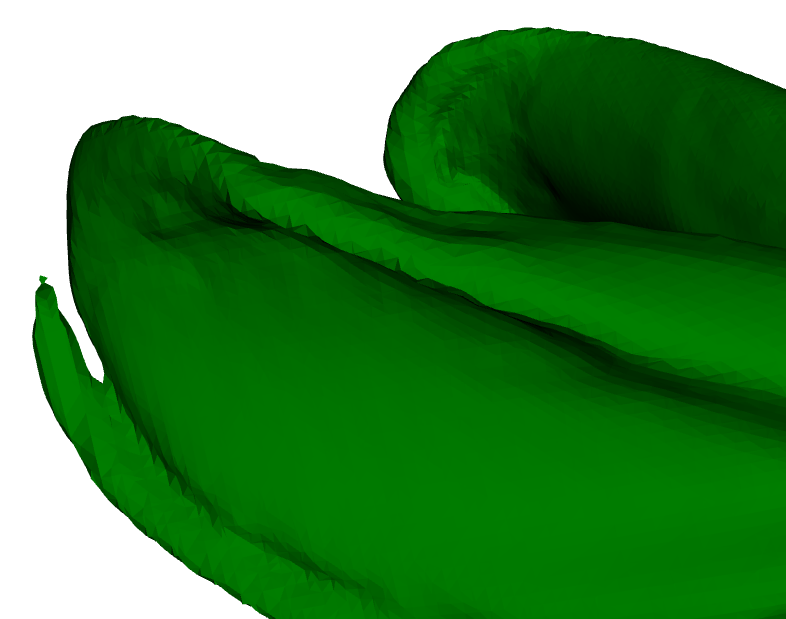
\includegraphics[max width=.5\linewidth, max height=.25\textheight, keepaspectratio]
				{img/bunny_ear}
			%\Imagen{img/bunny_ear}
			\caption[Acercamiento a la oreja derecha de \texttt{bunny}]{\label{fig:bun_ear}Acercamiento a la oreja derecha de \texttt{bunny}.}
		\end{figure}

		\begin{figure}
			%\Imagen{img/drill_drops}
			\centering
			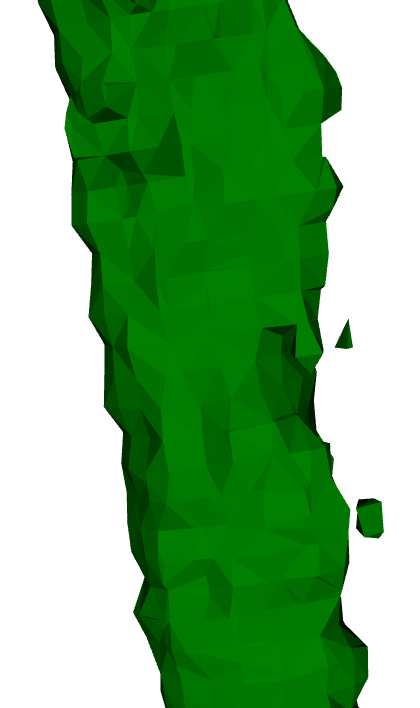
\includegraphics[max width=.5\linewidth, max height=.25\textheight, keepaspectratio]
				{img/drill_drops}
			\caption[Acercamiento a la mecha de \texttt{drill}]{\label{fig:drill_drops}Acercamiento a la mecha de \texttt{drill}.}
		\end{figure}

		\begin{figure}
			%\Imagen{img/drill_drops}
			\centering
			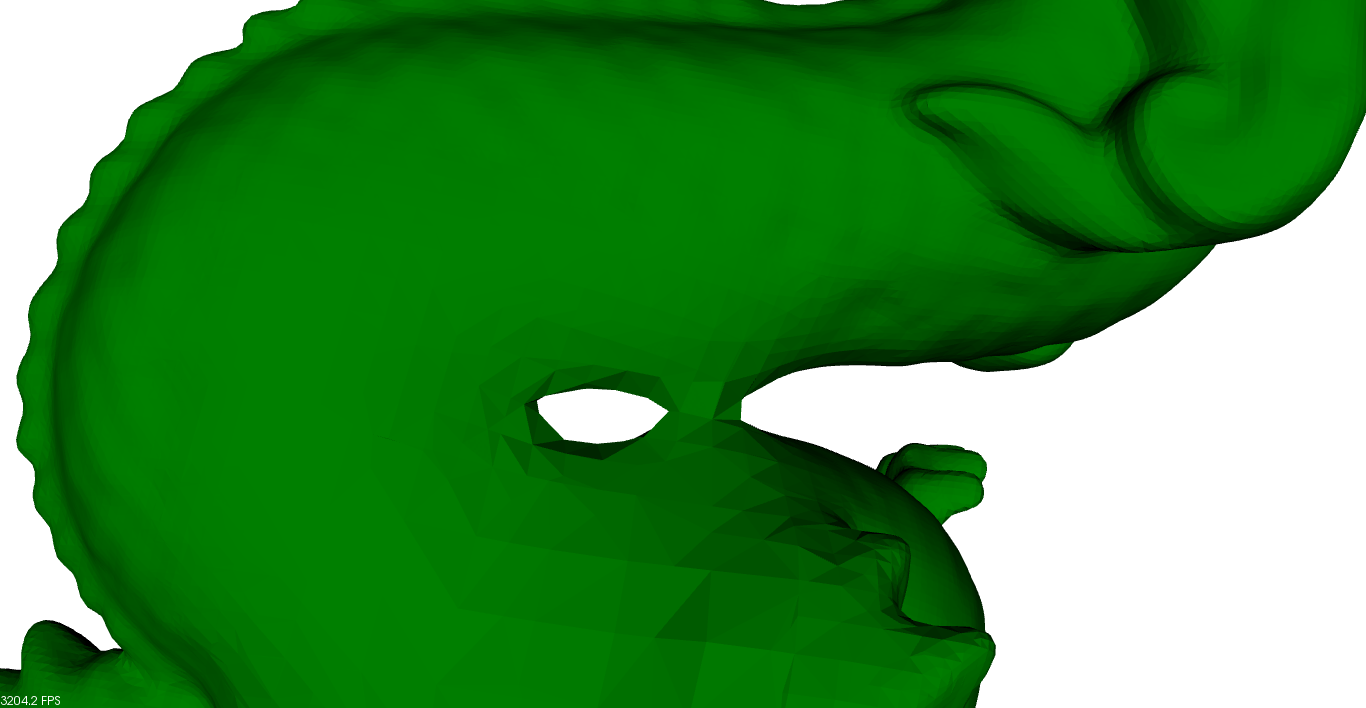
\includegraphics[max width=.5\linewidth, max height=.25\textheight, keepaspectratio]
				{img/dragon_belly}
			\caption[Acercamiento al vientre de \texttt{dragon}]{\label{fig:dragon_belly}Acercamiento al vientre de \texttt{dragon}.}
		\end{figure}

		\begin{figure}
			\centering
			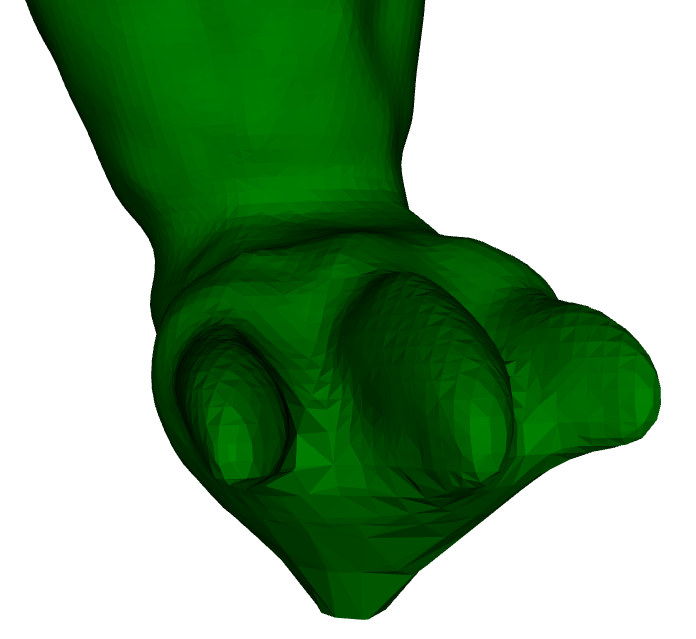
\includegraphics[max width=.5\linewidth, max height=.25\textheight, keepaspectratio]
				{img/arma_foot}
			%\Imagen{img/arma_foot}
			\caption[Acercamiento a la base de apoyo de \texttt{armadillo}]{\label{fig:base}Acercamiento a la base de apoyo de \texttt{armadillo}. Se observa un estiramiento hacia abajo debido al uso de condiciones de borde Neumann.}
		\end{figure}

		%trabajo futuro (advancing front)
		%Para evitar la divergencia es necesario definir una superficie de
		%soporte considerando todo el contorno del hueco, de forma de asegurar
		%que los nuevos puntos no excedan los límites del hueco.

	\section{Tiempo de ejecución}
	Para cada modelo se midieron los tiempos de ejecución requeridos por cada módulo de la reconstrucción
	sobre una PC
	Intel(R) Core(TM) i5-2500 CPU @ 3.30GHz
	con 8GB de RAM
	corriendo en un solo hilo.

		Se observa que la etapa de registración
		es responsable de la mayor parte del costo computacional, sobre todo al aumentar
		la cantidad de puntos en las capturas (cuadro~\ref{tab:reconstr_time}).
		En el cuadro~\ref{tab:reg_time} se muestran
		los tiempos de ejecución promedio, discriminados en la alineación
		inicial y el refinamiento posterior.
		El orden $\bigO\left(n^2\right)$ de la alineación inicial se debe a la búsqueda
		entre todos los pares de puntos para establecer las correspondencias (figura~\ref{fig:registration_order}).
		%Si bien los tiempos no son considerables, pueden reducirse al mejorar
		%la selección inicial de puntos y realizar la búsqueda de las
		%correspondencias de forma más eficiente.
		\begin{table}
	\centering
	\begin{tabular}{l*{6}{r}}
		\toprule
		Modelo                 & Puntos   & Capturas  &  Registración & Fusión   & Rellenado & Total\\
		\midrule
		armadillo back         &  25e3    &   11      &   84.4308        & 10.759  &  8.562  & 103.752\\
		armadillo head         &  25e3    &   12      &   114.4926       & 12.501  &  9.892  & 136.886\\
		armadillo head offset  &  25e3    &   11      &   100.7846       & 11.987  &  9.718  & 122.490\\
		armadillo stand        &  25e3    &   12      &   102.3553       & 12.145  &  9.498  & 123.998\\
		armadillo stand flip   &  25e3    &   11      &   101.7061       & 12.958  &  9.280  & 123.944\\
		\midrule
		bunny                  &  35e3    &   6       &    92.2872       & 11.246  &  11.862 & 115.395\\
		\midrule
		dragon side            &  20e3    &   15      &   90.5427        & 14.021  &  8.086  & 112.650\\
		dragon stand           &  30e3    &   15      &   180.8010       & 23.485  &  12.680 & 216.966\\
		dragon up              &  30e3    &   15      &   164.1075       & 18.469  &  9.669  & 192.245\\
		\midrule
		drill                  &   4e3    &   12      &   4.3172         & 1.988   &  4.176  & 10.481 \\
		\midrule
		happy back             &  45e3    &   15      &   343.2705       & 29.618  &  7.528  & 380.417\\
		happy side             &  45e3    &   15      &   452.5830       & 32.588  &  8.361  & 493.532\\
		happy stand            &  75e3    &   15      &   907.2930       & 44.570  &  10.929 & 962.792\\
		\bottomrule
	\end{tabular}
	\caption[Tiempo de reconstrucción]{\label{tab:reconstr_time}Tiempo de reconstrucción por cada modelo (en segundos).}
\end{table}



		\begin{table}
	\centering
	\begin{tabular}{l*{4}{c}}
		\toprule
		Modelo                 &  Puntos  &   Inicial (s)  &   ICP  (s)  &  Total  (s)\\
		\midrule
		armadillo\\
		{\Em}back         &  25e3    &       7.05694    &   0.618592  &    7.67553\\
		{\Em}head         &  25e3    &       8.94947    &   0.591576  &    9.54105\\
		{\Em}head offset  &  25e3    &       8.62241    &   0.539835  &    9.16224\\
		{\Em}stand        &  25e3    &       7.98686    &   0.542746  &    8.52961\\
		{\Em}stand flip   &  25e3    &       8.69949    &   0.546518  &    9.24601\\
		\midrule
		bunny                  &  35e3    &       14.0323    &   1.348890  &    15.3812\\
		\midrule
		dragon\\
		{\Em}side            &  20e3    &       5.52965    &   0.506529  &    6.03618\\
		{\Em}stand           &  30e3    &       11.3732    &   0.680195  &    12.0534\\
		{\Em}up              &  30e3    &       10.3322    &   0.608282  &    10.9405\\
		\midrule
		drill                  &   4e3    &       0.26898    &   0.090796  &    0.35977\\
		\midrule
		happy\\
		{\Em}back             &  45e3    &       21.2702    &   1.614520  &    22.8847\\
		{\Em}side             &  45e3    &       29.1103    &   1.061880  &    30.1722\\
		{\Em}stand            &  75e3    &       59.3281    &   1.158030  &    60.4862\\
		\bottomrule
	\end{tabular}
	\caption[Tiempos de ejecución promedio para la registración]{\label{tab:reg_time}Tiempos de ejecución promedio para la
	registración de a pares en los distintos modelos.}
\end{table}


		\begin{figure}
			\centering
			\begin{tikzpicture}[gnuplot]
%% generated with GNUPLOT 5.4p0 (Lua 5.4; terminal rev. Jun 2020, script rev. 114)
%% Thu 27 Aug 2020 10:08:06 PM -03
\gpmonochromelines
\path (0.000,0.000) rectangle (12.500,8.750);
\gpcolor{color=gp lt color border}
\gpsetlinetype{gp lt border}
\gpsetdashtype{gp dt solid}
\gpsetlinewidth{1.00}
\draw[gp path] (1.504,0.985)--(1.684,0.985);
\draw[gp path] (11.947,0.985)--(11.767,0.985);
\node[gp node right] at (1.320,0.985) {$10^{-2}$};
\draw[gp path] (1.504,1.546)--(1.594,1.546);
\draw[gp path] (11.947,1.546)--(11.857,1.546);
\draw[gp path] (1.504,1.874)--(1.594,1.874);
\draw[gp path] (11.947,1.874)--(11.857,1.874);
\draw[gp path] (1.504,2.107)--(1.594,2.107);
\draw[gp path] (11.947,2.107)--(11.857,2.107);
\draw[gp path] (1.504,2.288)--(1.594,2.288);
\draw[gp path] (11.947,2.288)--(11.857,2.288);
\draw[gp path] (1.504,2.435)--(1.594,2.435);
\draw[gp path] (11.947,2.435)--(11.857,2.435);
\draw[gp path] (1.504,2.560)--(1.594,2.560);
\draw[gp path] (11.947,2.560)--(11.857,2.560);
\draw[gp path] (1.504,2.668)--(1.594,2.668);
\draw[gp path] (11.947,2.668)--(11.857,2.668);
\draw[gp path] (1.504,2.764)--(1.594,2.764);
\draw[gp path] (11.947,2.764)--(11.857,2.764);
\draw[gp path] (1.504,2.849)--(1.684,2.849);
\draw[gp path] (11.947,2.849)--(11.767,2.849);
\node[gp node right] at (1.320,2.849) {$10^{-1}$};
\draw[gp path] (1.504,3.410)--(1.594,3.410);
\draw[gp path] (11.947,3.410)--(11.857,3.410);
\draw[gp path] (1.504,3.738)--(1.594,3.738);
\draw[gp path] (11.947,3.738)--(11.857,3.738);
\draw[gp path] (1.504,3.971)--(1.594,3.971);
\draw[gp path] (11.947,3.971)--(11.857,3.971);
\draw[gp path] (1.504,4.152)--(1.594,4.152);
\draw[gp path] (11.947,4.152)--(11.857,4.152);
\draw[gp path] (1.504,4.299)--(1.594,4.299);
\draw[gp path] (11.947,4.299)--(11.857,4.299);
\draw[gp path] (1.504,4.424)--(1.594,4.424);
\draw[gp path] (11.947,4.424)--(11.857,4.424);
\draw[gp path] (1.504,4.532)--(1.594,4.532);
\draw[gp path] (11.947,4.532)--(11.857,4.532);
\draw[gp path] (1.504,4.628)--(1.594,4.628);
\draw[gp path] (11.947,4.628)--(11.857,4.628);
\draw[gp path] (1.504,4.713)--(1.684,4.713);
\draw[gp path] (11.947,4.713)--(11.767,4.713);
\node[gp node right] at (1.320,4.713) {$10^{0}$};
\draw[gp path] (1.504,5.274)--(1.594,5.274);
\draw[gp path] (11.947,5.274)--(11.857,5.274);
\draw[gp path] (1.504,5.602)--(1.594,5.602);
\draw[gp path] (11.947,5.602)--(11.857,5.602);
\draw[gp path] (1.504,5.835)--(1.594,5.835);
\draw[gp path] (11.947,5.835)--(11.857,5.835);
\draw[gp path] (1.504,6.016)--(1.594,6.016);
\draw[gp path] (11.947,6.016)--(11.857,6.016);
\draw[gp path] (1.504,6.163)--(1.594,6.163);
\draw[gp path] (11.947,6.163)--(11.857,6.163);
\draw[gp path] (1.504,6.288)--(1.594,6.288);
\draw[gp path] (11.947,6.288)--(11.857,6.288);
\draw[gp path] (1.504,6.396)--(1.594,6.396);
\draw[gp path] (11.947,6.396)--(11.857,6.396);
\draw[gp path] (1.504,6.492)--(1.594,6.492);
\draw[gp path] (11.947,6.492)--(11.857,6.492);
\draw[gp path] (1.504,6.577)--(1.684,6.577);
\draw[gp path] (11.947,6.577)--(11.767,6.577);
\node[gp node right] at (1.320,6.577) {$10^{1}$};
\draw[gp path] (1.504,7.138)--(1.594,7.138);
\draw[gp path] (11.947,7.138)--(11.857,7.138);
\draw[gp path] (1.504,7.466)--(1.594,7.466);
\draw[gp path] (11.947,7.466)--(11.857,7.466);
\draw[gp path] (1.504,7.699)--(1.594,7.699);
\draw[gp path] (11.947,7.699)--(11.857,7.699);
\draw[gp path] (1.504,7.880)--(1.594,7.880);
\draw[gp path] (11.947,7.880)--(11.857,7.880);
\draw[gp path] (1.504,8.027)--(1.594,8.027);
\draw[gp path] (11.947,8.027)--(11.857,8.027);
\draw[gp path] (1.504,8.152)--(1.594,8.152);
\draw[gp path] (11.947,8.152)--(11.857,8.152);
\draw[gp path] (1.504,8.260)--(1.594,8.260);
\draw[gp path] (11.947,8.260)--(11.857,8.260);
\draw[gp path] (1.504,8.356)--(1.594,8.356);
\draw[gp path] (11.947,8.356)--(11.857,8.356);
\draw[gp path] (1.504,8.441)--(1.684,8.441);
\draw[gp path] (11.947,8.441)--(11.767,8.441);
\node[gp node right] at (1.320,8.441) {$10^{2}$};
\draw[gp path] (1.504,0.985)--(1.504,1.165);
\draw[gp path] (1.504,8.441)--(1.504,8.261);
\node[gp node center] at (1.504,0.677) {$10^{4}$};
\draw[gp path] (4.648,0.985)--(4.648,1.075);
\draw[gp path] (4.648,8.441)--(4.648,8.351);
\draw[gp path] (6.487,0.985)--(6.487,1.075);
\draw[gp path] (6.487,8.441)--(6.487,8.351);
\draw[gp path] (7.791,0.985)--(7.791,1.075);
\draw[gp path] (7.791,8.441)--(7.791,8.351);
\draw[gp path] (8.803,0.985)--(8.803,1.075);
\draw[gp path] (8.803,8.441)--(8.803,8.351);
\draw[gp path] (9.630,0.985)--(9.630,1.075);
\draw[gp path] (9.630,8.441)--(9.630,8.351);
\draw[gp path] (10.329,0.985)--(10.329,1.075);
\draw[gp path] (10.329,8.441)--(10.329,8.351);
\draw[gp path] (10.935,0.985)--(10.935,1.075);
\draw[gp path] (10.935,8.441)--(10.935,8.351);
\draw[gp path] (11.469,0.985)--(11.469,1.075);
\draw[gp path] (11.469,8.441)--(11.469,8.351);
\draw[gp path] (11.947,0.985)--(11.947,1.165);
\draw[gp path] (11.947,8.441)--(11.947,8.261);
\node[gp node center] at (11.947,0.677) {$10^{5}$};
\draw[gp path] (1.504,8.441)--(1.504,0.985)--(11.947,0.985)--(11.947,8.441)--cycle;
\node[gp node center,rotate=-270] at (0.292,4.713) {tiempo};
\node[gp node center] at (6.725,0.215) {puntos};
\gpsetpointsize{4.00}
\gp3point{gp mark 7}{}{(5.660,6.363)}
\gp3point{gp mark 7}{}{(5.660,6.539)}
\gp3point{gp mark 7}{}{(5.660,6.506)}
\gp3point{gp mark 7}{}{(5.660,6.448)}
\gp3point{gp mark 7}{}{(5.660,6.514)}
\gp3point{gp mark 7}{}{(7.186,6.926)}
\gp3point{gp mark 7}{}{(4.648,6.168)}
\gp3point{gp mark 7}{}{(6.487,6.728)}
\gp3point{gp mark 7}{}{(6.487,6.650)}
\gp3point{gp mark 7}{}{(8.325,7.247)}
\gp3point{gp mark 7}{}{(8.325,7.471)}
\gp3point{gp mark 7}{}{(10.642,8.034)}
\gpsetdashtype{gp dt 1}
\draw[gp path] (2.031,2.322)--(2.137,3.390)--(2.242,3.845)--(2.348,4.142)--(2.453,4.364)%
  --(2.559,4.543)--(2.664,4.694)--(2.770,4.825)--(2.875,4.940)--(2.981,5.044)--(3.086,5.139)%
  --(3.192,5.227)--(3.297,5.308)--(3.403,5.384)--(3.508,5.456)--(3.614,5.523)--(3.719,5.588)%
  --(3.825,5.649)--(3.930,5.708)--(4.036,5.765)--(4.141,5.820)--(4.247,5.872)--(4.352,5.923)%
  --(4.458,5.973)--(4.563,6.021)--(4.669,6.068)--(4.774,6.114)--(4.880,6.159)--(4.985,6.202)%
  --(5.090,6.245)--(5.196,6.287)--(5.301,6.329)--(5.407,6.369)--(5.512,6.409)--(5.618,6.448)%
  --(5.723,6.487)--(5.829,6.525)--(5.934,6.563)--(6.040,6.600)--(6.145,6.637)--(6.251,6.674)%
  --(6.356,6.710)--(6.462,6.746)--(6.567,6.781)--(6.673,6.816)--(6.778,6.851)--(6.884,6.885)%
  --(6.989,6.920)--(7.095,6.954)--(7.200,6.988)--(7.306,7.021)--(7.411,7.055)--(7.517,7.088)%
  --(7.622,7.121)--(7.728,7.154)--(7.833,7.187)--(7.939,7.220)--(8.044,7.252)--(8.150,7.285)%
  --(8.255,7.317)--(8.361,7.349)--(8.466,7.382)--(8.571,7.414)--(8.677,7.446)--(8.782,7.478)%
  --(8.888,7.510)--(8.993,7.542)--(9.099,7.573)--(9.204,7.605)--(9.310,7.637)--(9.415,7.669)%
  --(9.521,7.700)--(9.626,7.732)--(9.732,7.764)--(9.837,7.795)--(9.943,7.827)--(10.048,7.859)%
  --(10.154,7.890)--(10.259,7.922)--(10.365,7.954)--(10.470,7.985)--(10.576,8.017)--(10.681,8.049)%
  --(10.787,8.081)--(10.892,8.112)--(10.998,8.144)--(11.103,8.176)--(11.209,8.208)--(11.314,8.240)%
  --(11.420,8.272)--(11.525,8.304)--(11.631,8.336)--(11.736,8.368)--(11.842,8.400)--(11.947,8.432);
\gpsetdashtype{gp dt solid}
\draw[gp path] (1.504,8.441)--(1.504,0.985)--(11.947,0.985)--(11.947,8.441)--cycle;
%% coordinates of the plot area
\gpdefrectangularnode{gp plot 1}{\pgfpoint{1.504cm}{0.985cm}}{\pgfpoint{11.947cm}{8.441cm}}
\end{tikzpicture}
%% gnuplot variables

			\caption{\label{fig:registration_order}Tiempo de ejecución de la registración, ajustado a una función de orden $\bigO\left(n^2\right)$.}
		\end{figure}
